\documentclass[usenatbib]{mn2e}
\usepackage{graphicx}
\usepackage{bm}
\usepackage{fixltx2e}
\usepackage{astrobib_mnras2e}
%\usepackage{lineno}

% Filler text
\usepackage{lipsum}

\begin{document}
\topmargin-1cm
%\linenumbers

%Make my life significantly easier
\newcommand{\vx}{{\bm x}}
\newcommand{\vr}{{\bm r}}
\newcommand{\vdx}{{\bm dx}}
\newcommand{\vy}{{\bm y}}
\newcommand{\bin}{\Theta}


\title[Geometric Integrals for Correlation Functions]
{On Calculating the Geometric Integrals in Correlation Function Estimators}
\author[Parejko\&Padmanabhan]{John Parejko$^{1}$, Nikhil Padmanabhan$^{1}$ or
reversed \\
$^{1}$ Dept. of Physics, Yale University, New Haven, CT 06511 \\
}

\date{\today}
\maketitle

\begin{abstract}
  We present a quasi-Monte Carlo technique for computing the geometric integrals - $RR$ and $DR$ - that appear
  in pair-counted correlation function estimators. We demonstrate that this technique can accelerate the convergence of
  these integrals, substantially reducing the number of random points required
  to reach a desired error target. MAYBE PUT IN EXACT SCALINGS, DEPENDING ON
  WHAT WE FIND??? We also present a simplification for surveys with separable
  angular and radial window functions. ????
\end{abstract}

\section{Introduction}

The correlation function is one of the fundamental measurements in
characterizing the distribution of galaxies, both on small and large scales.
Given its importance, ????? DISCUSS FAST METHODS HERE ETC ETC ETC ???

BRIEF DESCRIPTION OF THIS WORK

This paper is organized as follows : Sec.~\ref{sec:RR} introduces the $RR$
integral, and presents the usual method by which it is estimated. We then
introduce our suggested technique for calculating this integral, constrasting it
with the usual calculation in a series of three toy problems. We then summarize
the algorithm in Sec.~\ref{sec:alg} and present a realistic examples from
the DEEP2 DR4 (CITE???) survey. We then present an
important simplification applicable to surveys with separable 
angular and radial selection functions in Sec.~\ref{sec:sep}.
We continue by extending our algorithm to the $DR$ integral in
Sec.~\ref{sec:DR}. Appendix~\ref{sec:review} reviews the basics of Monte Carlo and quasi-Monte
Carlo integration techniques, and gathers together results used in this work.

A note on the nomenclature used in the paper. Vectors are denoted as ($\vx$),
with their components specified as $x_{i}$. We also define a bin function
$\bin(\vx,\vy)$ which is $1$ if the separation between $\vx$ and $\vy$
corresponds to the bin of interest, and zero otherwise. 

\section{The RR Integral}
\label{sec:RR}

We start by reviewing the basics of galaxy correlation function estimation, as 
is most commonly used in large-scale structure work today. We then introduce 
our modifications in a series of toy examples, that highlight both the algorithm
and the differences with the traditional approach.

\subsection{Correlation Function Estimators and their Standard Calculation}

The galaxy two-point correlation $\xi(r)$ is defined as the fractional excess
over a uniform distribution in the number of galaxy pairs separated by a
distance $r$ from one another. The most commonly used estimator is the
Landy-Szalay (CITE???) estimator :
\begin{equation}
\xi = \frac{DD - 2 DR + RR}{RR}
\end{equation}
where $\xi$ here represents the correlation function in a particular separation
bin (appropriately averaged) and $DD$ is the number of galaxy pairs that fall in
that bin. This raw number of pairs must be scaled and corrected for the effects
of the survey selection function. The $DR$ and $RR$ terms represent this correction. 
$RR$ is the expected number of pairs
if the galaxies were homogeously distributed according to the survey selection
function, while $DR$ is the expected number of pairs around the actual galaxies
themselves. If we consider the survey selection function $n(\vx)$ normalized
by the volume integral
\begin{equation}
N = \int d\vx\,n(\vx)
\end{equation}
where $N$ is the observed number of galaxies, then 
\begin{equation}
RR = \int d\vx_1  \int d\vx_2 \,n(\vx_1) n(\vx_2) \bin(\vx,\vy) \,\,,
\label{eq:RRdef}
\end{equation}
and 
\begin{equation}
DR = \sum_{i=1}^{N} \int d\vx_1 \,n(\vx_1) \bin(\vx_1, \vx_{g,i}) \,\,
\label{eq:DRdef}
\end{equation}
where the sum for $DR$ runs over the $N$ galaxy positions $\vx_{g,i}$. 
Note that for an $n$-dimensional galaxy distribution, the $RR$ integral is
$2n$-dimensional, while $DR$ is $n$-dimensional. In what follows, it will be
convenient to scale $DR$ and $RR$ as defined by $1/N^2$, equivalent to
normalizing the selection function by $\int d\vx\,n(\vx)=1$. For simplicity, we
refer to these as $DR$ and $RR$ as well. 

In what follows, it is important to remember that both $DR$ and $RR$ are purely
geometric quantities and do not have any intrinsic statistical fluctuations.
These therefore should be estimated at a high enough accuracy to introduce no
additional errors to the correlation function estimate. 

\subsection{Calculating RR}

Given the complexity of survey selection functions, these integrals are most
conveniently estimated by Monte-Carlo techniques. We continue to adopt this
approach here, and only depart in the details of our implementation. We focus on
the $RR$ calculation here, and discuss the $DR$ calculation in Sec.???. 

The traditional approach to calculating $RR$ is to lay down a set random points
according to the survey selection function and then to count the number of pairs
when correlating this random catalog with itself. This approach has much to
recommend it : it is identical to the $DD$ calculation and therefore
conceptually simple to implement, and the random catalogs so created are a
convenient and portable representation of the survey selection function.
However, the number of random points needs to be significantly larger than the
number of data points to prevent the estimation error in $RR$ from contributing
to the error in $\xi$; factors of 50 to 100 times the data sample are relatively
commonly used. A result of this is that the calculation of the correlation
function is immediately dominated by the $RR$ pair counting, and significant
effort has been expended to speed up this calculation, both with algorithmic
improvements (CITES???) and parallelization (CITES????).

\begin{figure*}
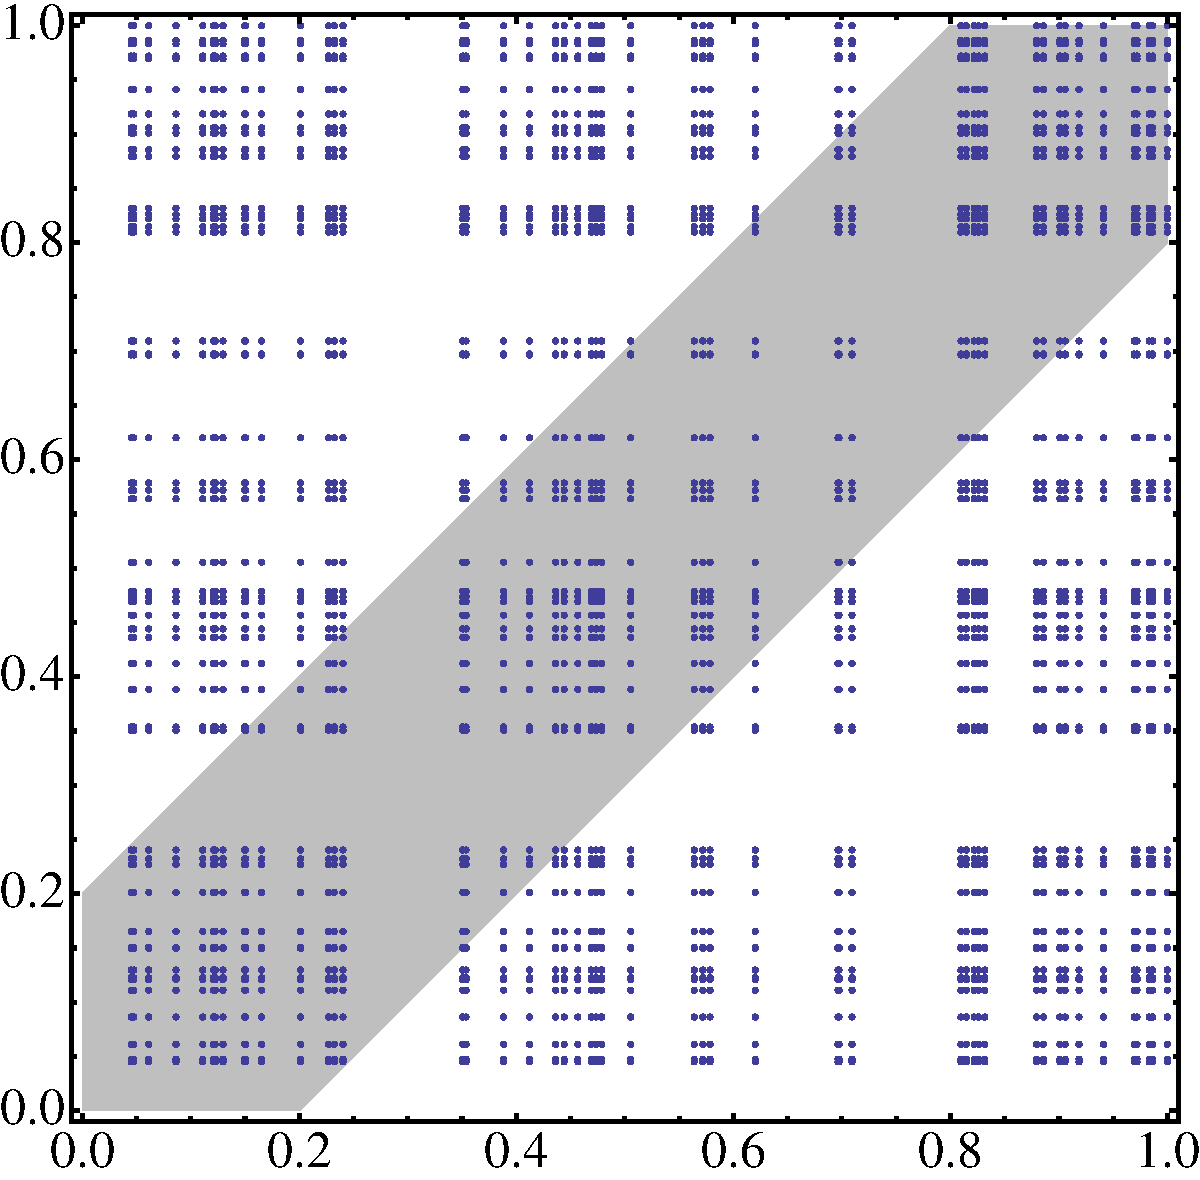
\includegraphics[width=1.5in]{plots/grid1d-1}
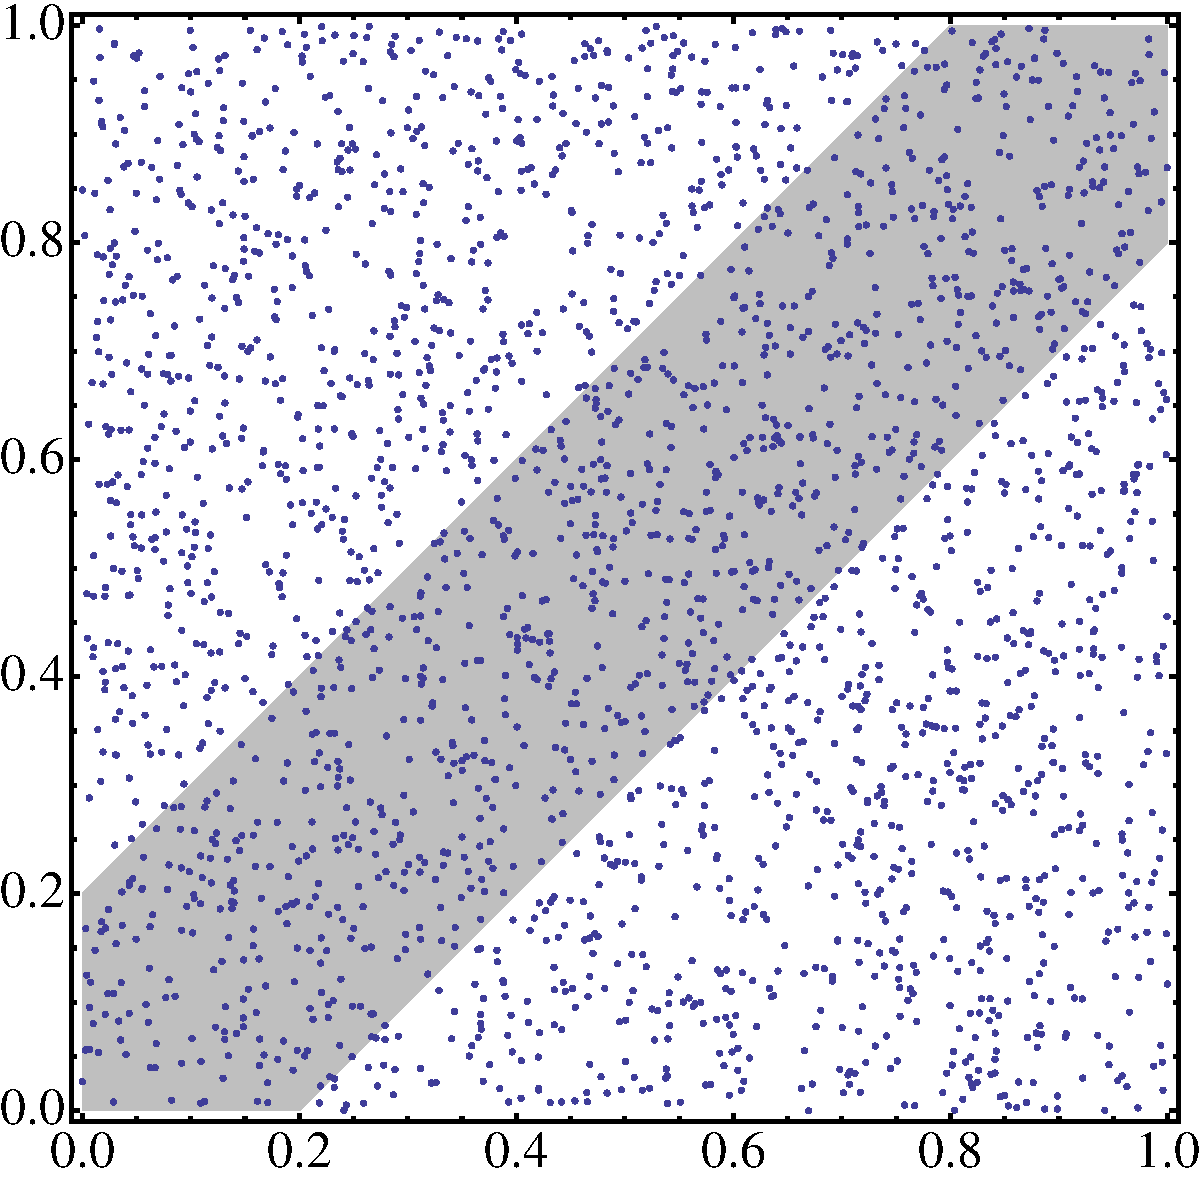
\includegraphics[width=1.5in]{plots/grid1d-2}
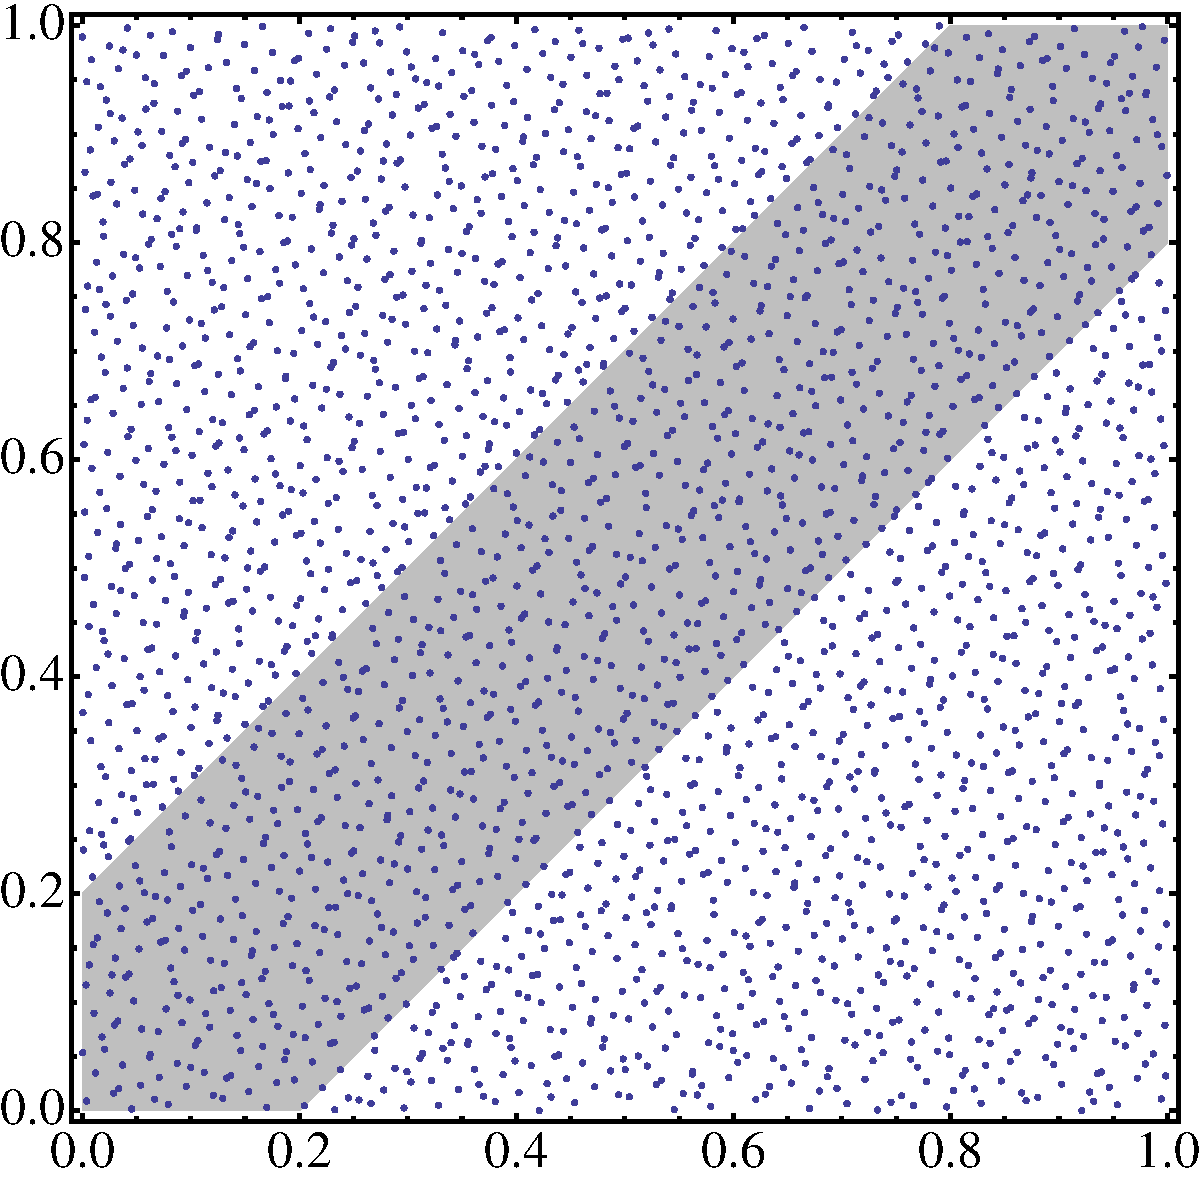
\includegraphics[width=1.5in]{plots/grid1d-3}
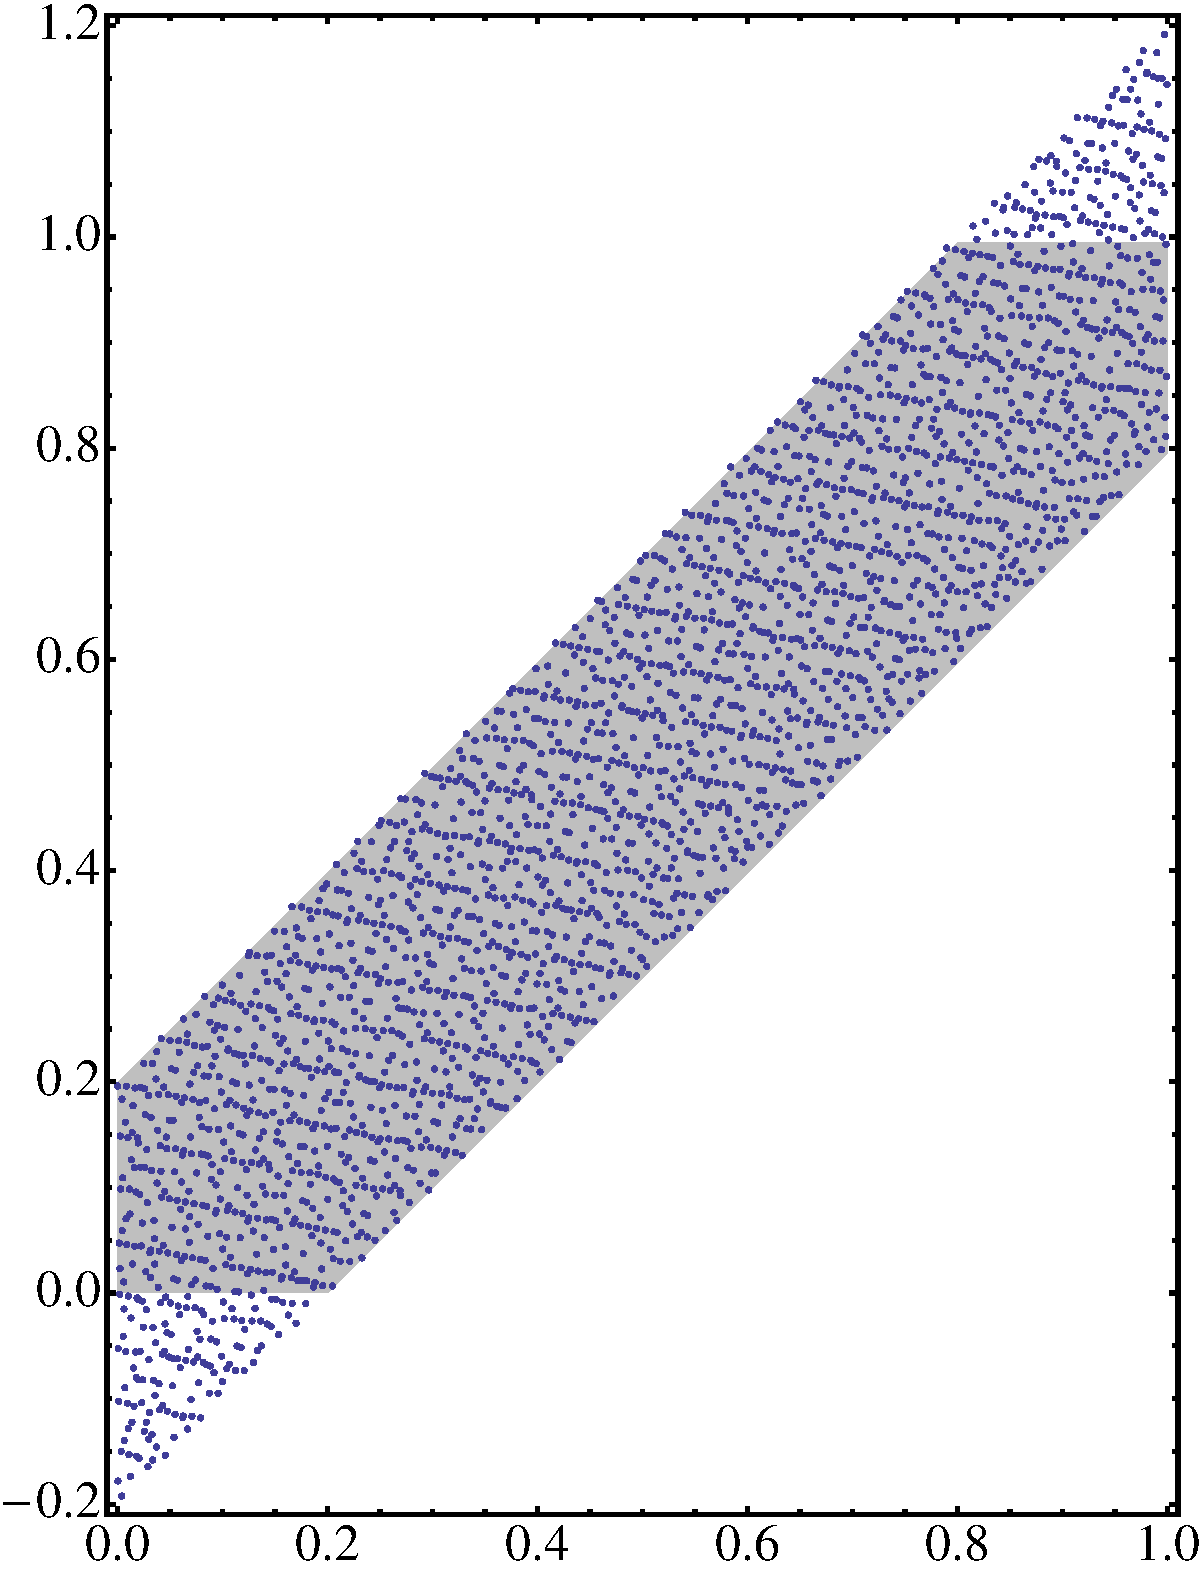
\includegraphics[width=1.5in]{plots/grid1d-4}
\caption{Computing $RR$ for a 1D survey geometry on the unit interval
for points separated by 0.2. The area of the shaded region is the desired value
of $RR$. Starting from the left, the panels are (a) the traditional algorithm,
formed by the Cartesian product of a 1D random set, (b) pseudo-random 2D
numbers, (c) a 2D Niederreiter quasi-random sequence and (d) a 2D Niederreiter
sequence in position and displacement (see text). Note that the $y$-axis in the
last panel runs from -0.2 to 1.2 to account for points on the edges. The number
of points (pairs) in all panels is the same.}
\label{fig:grid1d}
\end{figure*}


The inefficiencies with this approach is clearly demonstrated by a toy example.
Consider a 1D survey geometry, and imagine we
needed to estimate $RR$ for points separated by less than a chosen distance. 
Fig.~\ref{fig:grid1d} graphically demonstrates this for a survey defined on
the unit interval, and a separation distance of 0.2. Calculating $RR$ is
equivalent to the problem of calculating the area of the shaded region. The
leftmost panel illustrates the algorithm as described above. Since the pairs are
the Cartesian product of the random set, they arrange themselves onto a grid,
and cover the 2D integral domain very non-uniformly. As we will see explicitly
below, this adversly affects the convergence rate of this algorithm below,
scaling much slower than the $\sqrt{N_{\rm pairs}}$ that one would expect for a
random sequence. 

Our first improvement is shown in the second panel - we simply
randomly\footnote{Technically, pseudo-randomly, since the random number
generator is completely deterministic given a starting seed. We use the GSL
implementation of the Mersenne Twister throughout this paper.} distribute the
points over the full integration domain.
Both panels have the same number of points sampling the integration domain, and the difference in
coverage is apparent. This is {\it not} equivalent to generating two separate
random sets and correlating them - we are sampling points from the underlying $2n$ dimensional 
space (2D in this case). We expect this to scale as
$\sqrt{N_{\rm pairs}}$ (see below). 

\subsection{A Spherical Cap and a Unit Cube}

\lipsum[1-3]

\begin{figure}
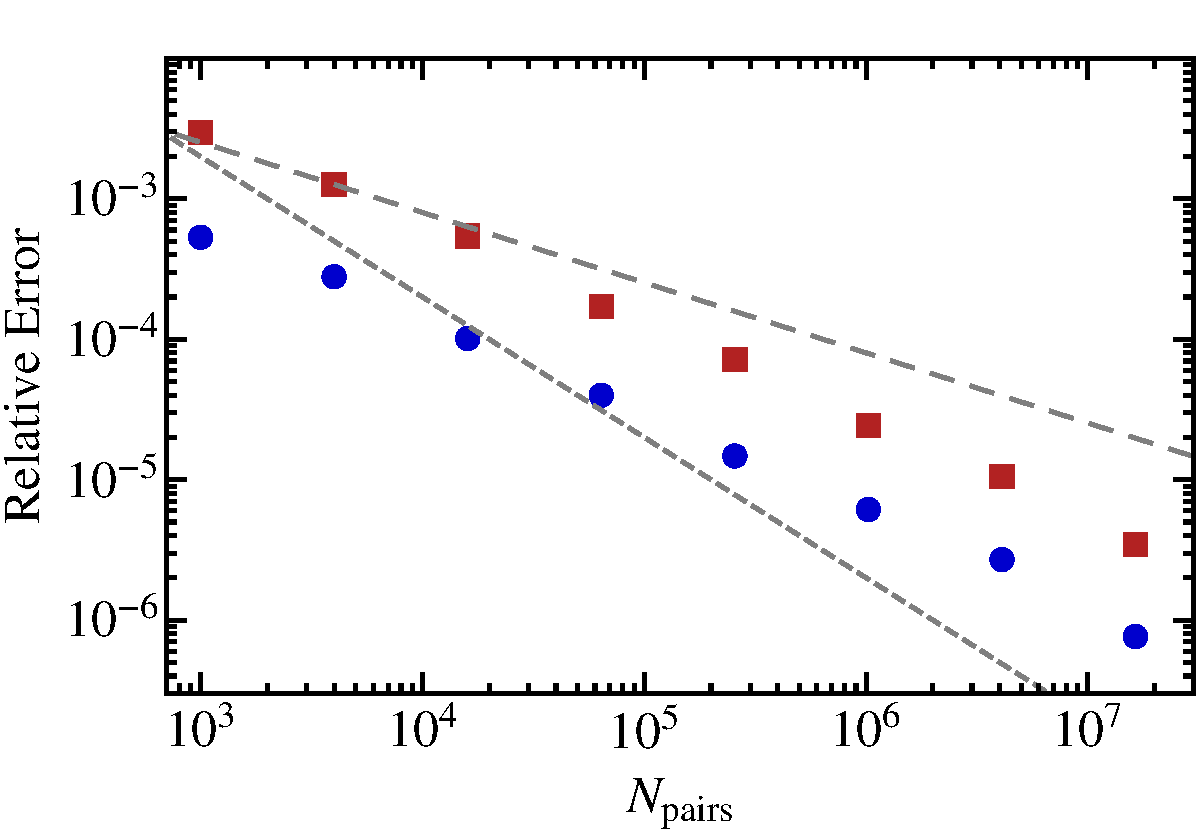
\includegraphics[width=3in]{plots/cap2d}
\caption{???The scaling of the relative error in RR for a spherical cap as a function of the number
of pairs. The cap is centered about the north pole, and extends down by
$60^{\circ}$. The circles and squares correspond to separations of points $<
0.1$ and $10$ degrees respectively. The long and short dashed lines are
$\propto N_{\rm pairs}^{-1/2}$ and $N_{\rm pairs}^{-1}$ respectively. The error
scaling is steeper than the $N^{-1/2}$ expected from purely random numbers.}
\label{fig:cap2d}
\end{figure}


\begin{figure}
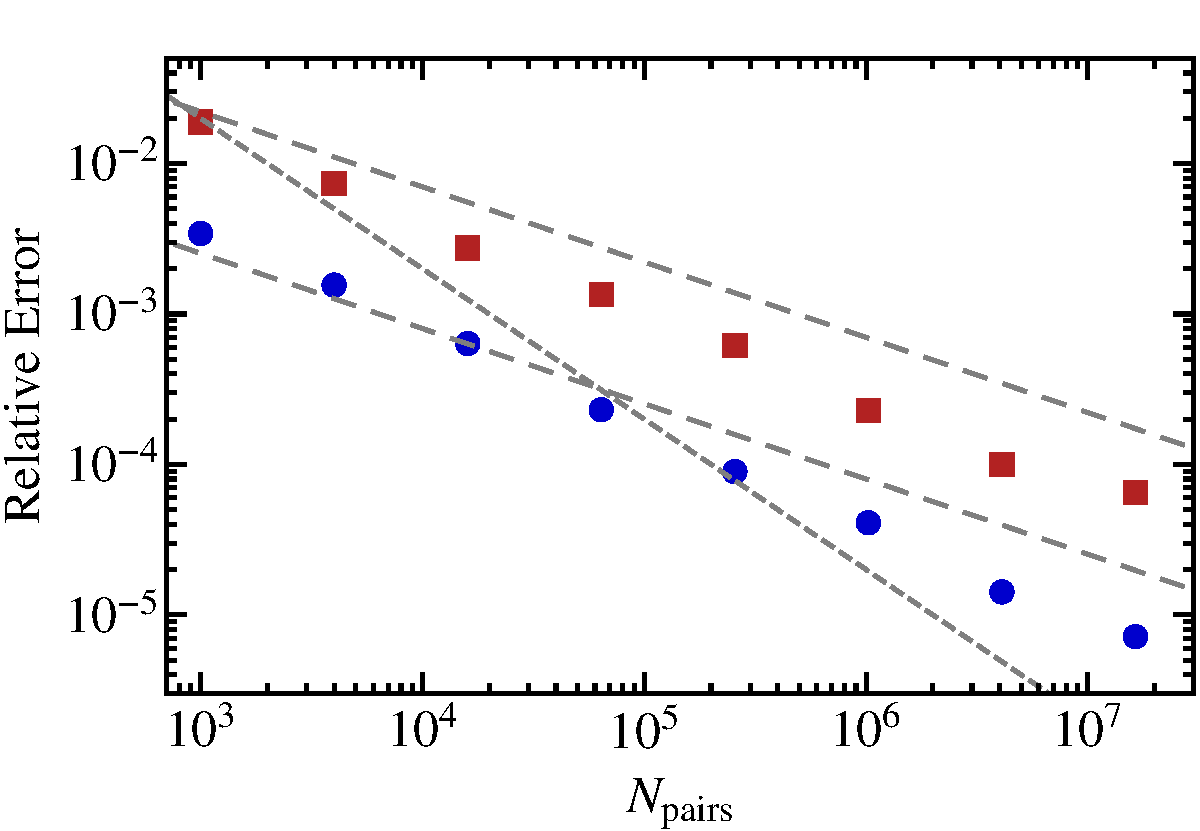
\includegraphics[width=3in]{plots/unit3d}
\caption{???The scaling of the relative error in RR for a unit cube as a
function of the number of pairs. The circles and squares correspond to radial
bins of $[0.015625,0.03125]$ and $[0.25,0.5]$ respectively.
The long and short dashed lines are $\propto N_{\rm pairs}^{-1/2}$ and $N_{\rm pairs}^{-1}$ respectively. The error
scaling is steeper than the $N^{-1/2}$ expected from purely random numbers.}
\label{fig:unit3d}
\end{figure}

\section{Real World Examples}

\subsection{The Algorithm Summarized}
\label{sec:alg}

PSEUDO-CODE HERE?????
\begin{enumerate}
  \item Generate a random vector in $[0,1)^{2n}$ .
  \begin{enumerate}
    \item Repeat the instructions in this group $N$ times.
    \item Generate a $2n$ dimensional element in $[0,1)^{2n}$ from a low
    discrepancy sequence.
    \item Shift it (mod 1) by the random vector stored above.
    \item Generate $\vx$ from the first $n$ elements and $\vdx$ from the last
    $n$.
    \item Generate $\vy$ from $\vx$ and $\vdx$. The most common rules are
    summarized below.
    \item Evaluate $n_1(\vx) n_2(\vy) \bin(\vx, \vy)$ and add to a running sum
    $\Sigma$.
  \end{enumerate}
  \item The estimate for $RR$ is then $\Sigma/N$ multiplied by the appropriate
  Jacobian factors from the variable transformations. 
  \item If desired, an error may be estimated by repeating this process and
  measuring the scatter. 
\end{enumerate}

COMMON VARIABLE TRANSFORMATIONS
\begin{itemize}
  \item $2D$ Cartesian space
  \item $2D$ Spherical coordinates
  \item $3D$ Cartesian space
\end{itemize}

\lipsum[1-3]

\subsection{Two Dimensions : The DEEP2 DR4 Survey Mask}

\begin{figure}
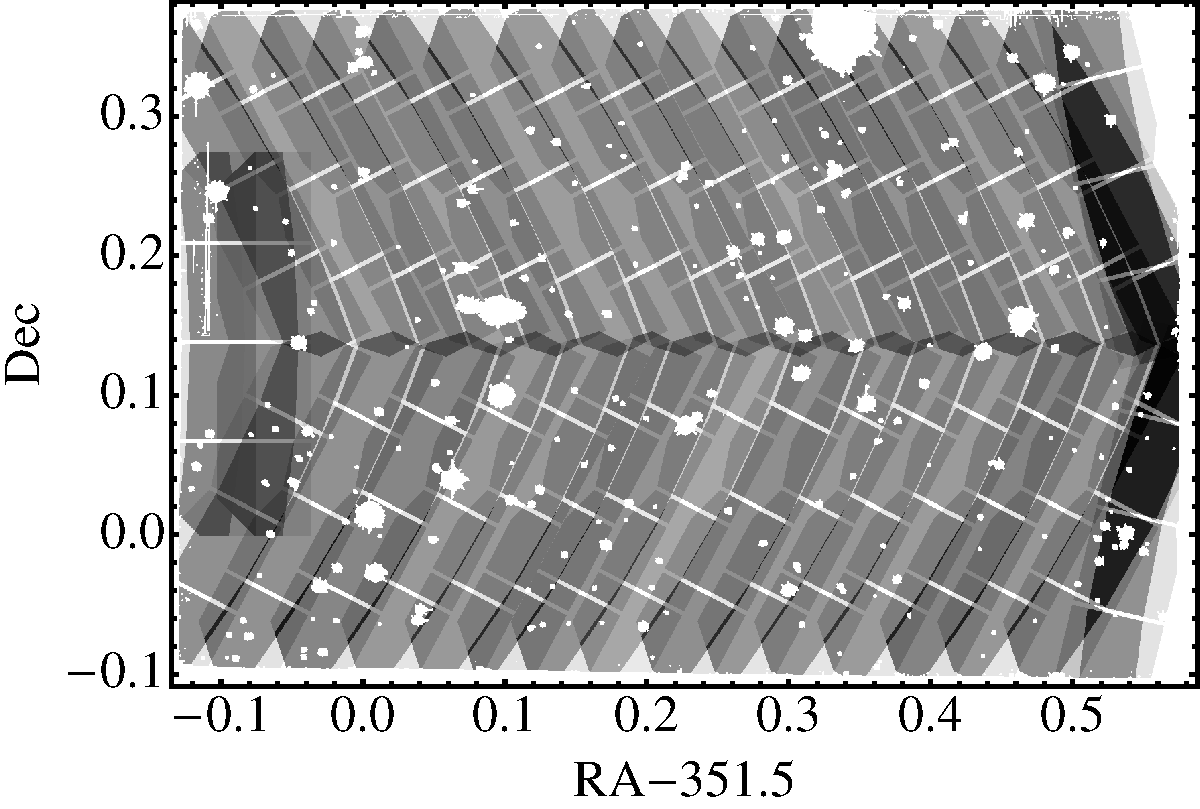
\includegraphics[width=3in]{plots/deep2mask}
\caption{The DEEP2 survey mask for the first pointing in field 3. The
completeness ranges from 0 (white) to 1 (black). }
\label{fig:deep2mask}
\end{figure}

\begin{figure}
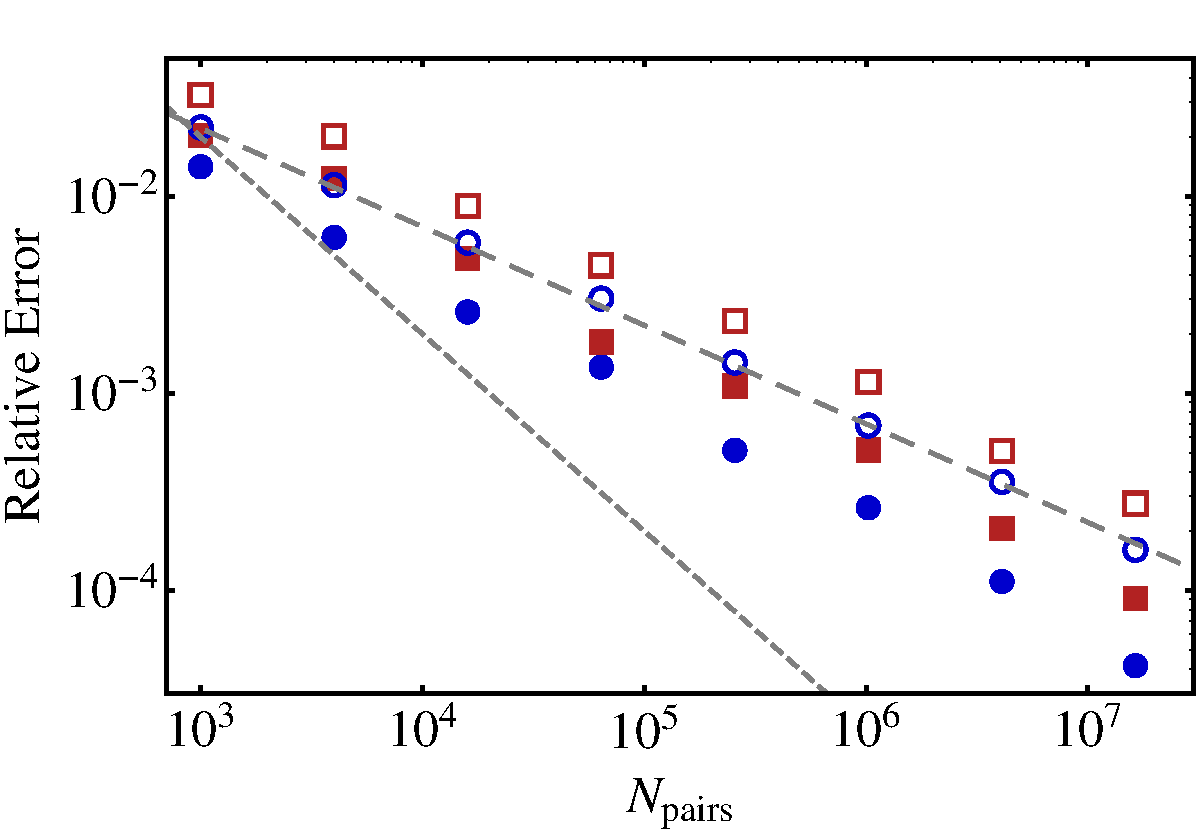
\includegraphics[width=3in]{plots/deep2rrcomp1}
\caption{???The scaling of the relative error in RR for the DEEP2 survey mask as
a function of the number of pairs. The circles and squares correspond to the
angular bins $[28.12,56.25]$ arcseconds and $[7.5,15]$ arcminutes respectively,
while the filled and open symbols compare a low discrepancy
sequence to pseudo-random numbers. The long and short dashed lines are
$\propto N_{\rm pairs}^{-1/2}$ and $N_{\rm pairs}^{-1}$ respectively. The low
discrepancy sequences outperform pseudo-random numbers both in the
absolute error as well as in the scaling with $N_{\rm pairs}$.}
\label{fig:deep2comp1}
\end{figure}

\begin{figure}
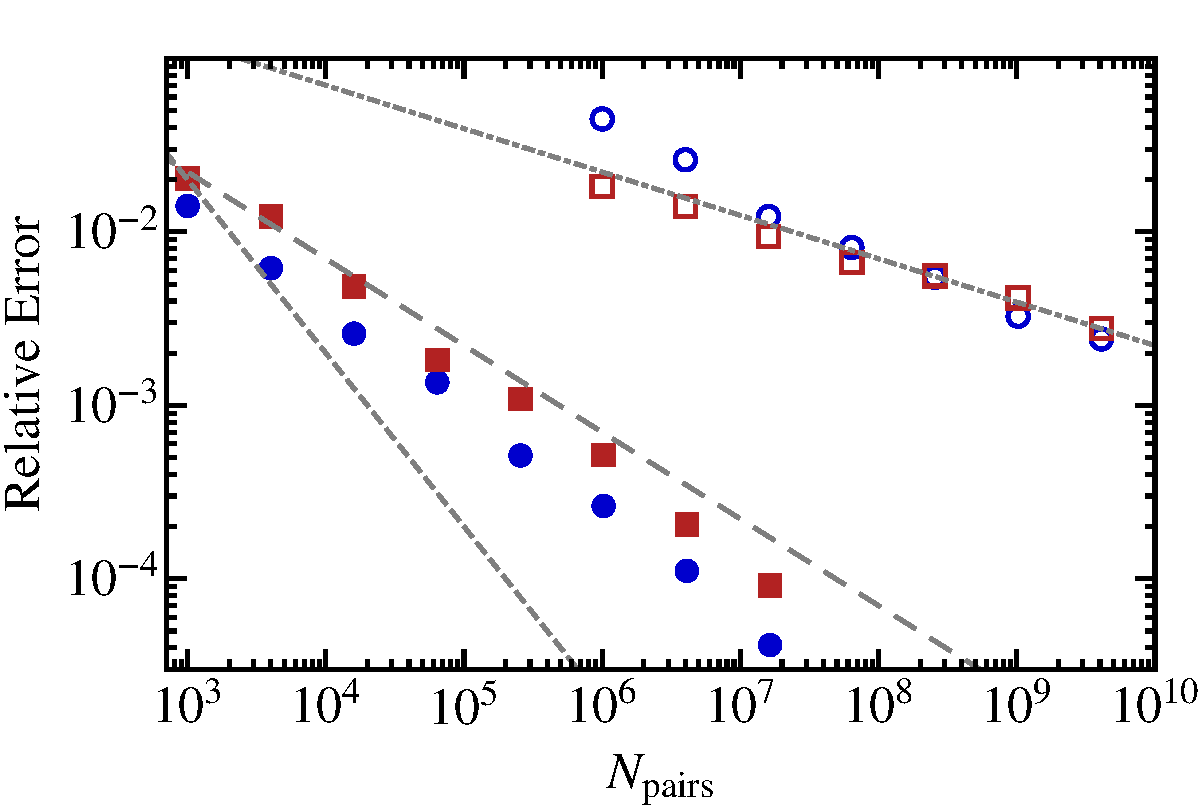
\includegraphics[width=3in]{plots/deep2rrcomp2}
\caption{The same as Fig.~\ref{fig:deep2comp1} except the open symbols are now
calculated using the traditional RR method. The dot-dashed line is $\propto
N_{\rm pairs}^{-1/4}$. The significant inefficiencies in the traditional
approach are clearly apparent here. }
\label{fig:deep2comp2}
\end{figure}

\begin{figure}
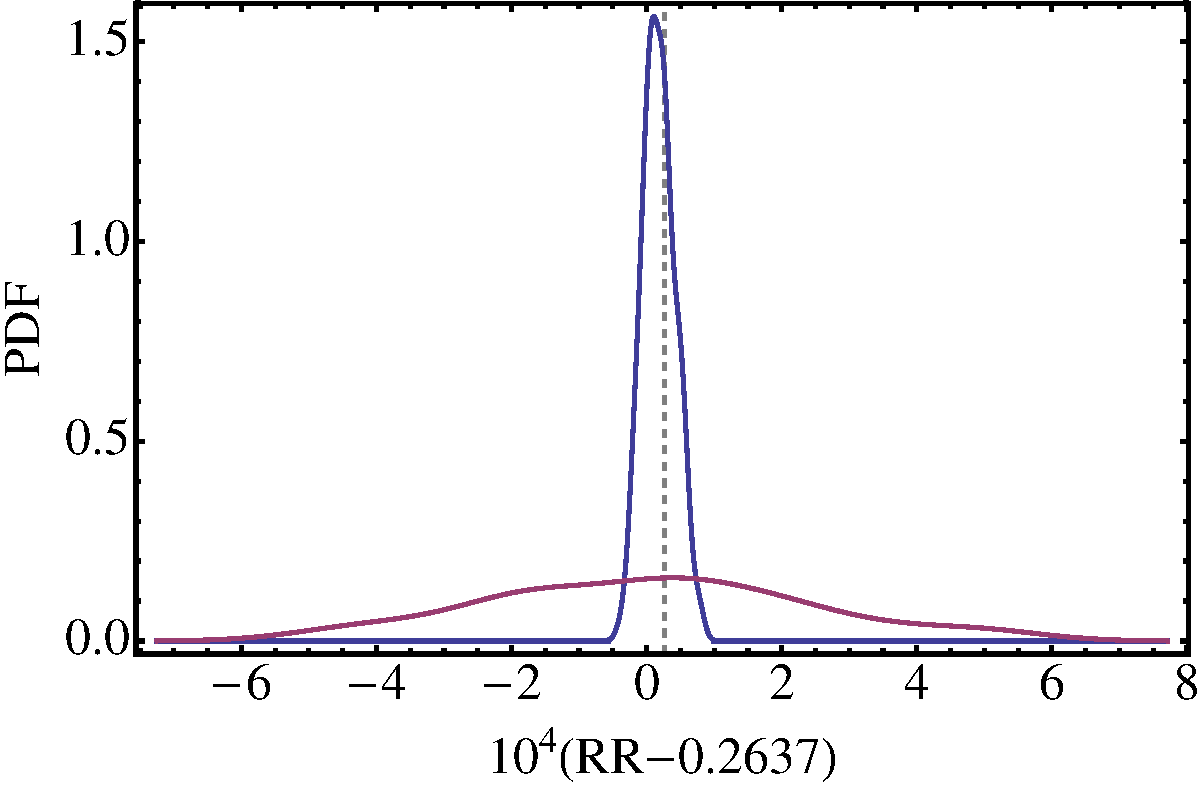
\includegraphics[width=3in]{plots/deep2rrhist}
\caption{????}
\label{fig:deep2comp2}
\end{figure}


\lipsum[1-3]

\subsection{Three Dimensions : The BOSS LOWZ sample}

\lipsum[1-3]

\subsubsection{Geometry}

\lipsum[1-3]

\subsection{Separable Window Functions}
\label{sec:sep}

\lipsum[1-3]

\section{The DR Integral}
\label{sec:DR}

\lipsum[1-3]

\section{Conclusions}
\label{sec:conclude}

\lipsum[1-3]

\section{Acknowledgments}


\end{document}




